\documentclass[10pt,a4paper,draft]{article}
\usepackage[utf8x]{inputenc}
\usepackage{ucs}
\usepackage[english]{babel}
\usepackage{multirow}
\usepackage{rotating}
\author{Lukáš Petrovický}
\title{RAS2012: Competition Entry}
\begin{document}

\maketitle

\begin{abstract}
This article describes an entry to the 2012 RAS Problem Solving Competition, concerning dispatching on multi-track territories. The entry is based on the Drools Planner, a Java-based solver. On a reasonably recent computer, the resulting algorithm is able to produce feasible results within a minute and has been fine-tuned to provide best results in under 3 minutes. Source code to the entry is open source and well documented.
\end{abstract}

\section{Introduction}

\section{Describing the solution}

\section{Implementation}

\section{Achieved results}

Running the algorithm described above 50 times over each data set, we have compiled a set of results, see Table \ref{table:result}. All these were reached within 3 minutes in a single-threaded run, using Intel i7 Q820 processor running Fedora 17 and 2 GB of heap space inside Java 7 runtime environment.

\begin{table}
\footnotesize
\caption{Submission performance per data set.}
\centering
\begin{tabular}{c||c|c|c|c|c}
\hline \hline
                 & Best                 & Q1                 & Q2                & Q3                & Worst \\ 
\hline
TOY & \$1074   & \$1074   & \$1074  & \$1074  & \$1074 \\
\hline
RDS1 & \$2056   & \$2251   & \$2561.5  & \$3385  & \$4628 \\
\hline
RDS2 & \$7895   & \$9270   & \$9851.5  & \$10600  & \$12462 \\
\hline
RDS3 & \$10257   & \$11194   & \$11816  & \$12396  & \$14135 \\
\end{tabular} 
\label{table:result} 
\end{table}

\begin{figure}
\centering
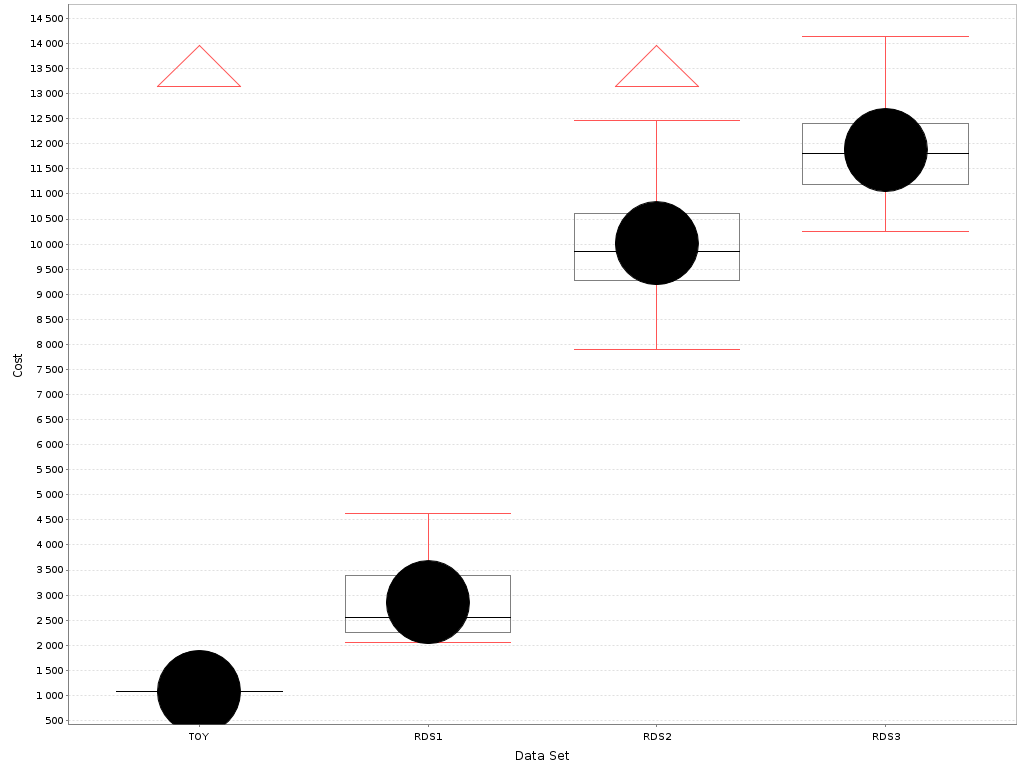
\includegraphics[width=120mm]{chart.png}
\caption{Plotting the data for the various resolved systems.}
\end{figure}

Please note that via the benchmarking functionality of Drools Planner, users may be able to fine-tune the algorithm to be focused either on providing better solutions or on faster turnaround times. Drools Planner even allows for retrieving the intermediate results of the algorithm and also modify the problem while it's being solved, which makes it the ideal tool for real-time planning.

For statistics of the resolved systems, see tables \ref{table:RASDATASET1}, \ref{table:RASDATASET2} and \ref{table:RASDATASET3} respectively. 

\section{Conclusion}

\appendix

\section{Resolved systems}

In this section, we show the best solutions reached for each data set. 

\begin{sidewaystable}
\footnotesize
\caption{Resolved system ``RAS DATA SET 1'', costing \$1199. Seed: 3458425443814323529.}
\centering
\begin{tabular}{c||c|c|c||c|c|c|c||c|c|c}
  \hline \hline
  &
  Unpref. & 
  Delay &
  Pty &
  Node &
  SA &
  Actual &
  Pty &
  TWT &
  Actual &
  Pty \\
      \hline
      \multirow{2}{*}{A1} &
      \multirow{2}{*}{0} &
      \multirow{2}{*}{0} &
      \multirow{2}{*}{0} &
      37 &
      3600 &
        3172.5 &
        0 &
      \multirow{2}{*}{5400} &
        \multirow{2}{*}{6106.5} &
        \multirow{2}{*}{0}
      \\
      \cline{5-8}
       &
       &
       &
       &
      39 &
      7800 &
        6106.5 &
        0 &
      
         &
        
      \\
      \hline
      \multirow{2}{*}{A2} &
      \multirow{2}{*}{0} &
      \multirow{2}{*}{1800} &
      \multirow{2}{*}{300} &
      37 &
      7800 &
        7924.742 &
        0 &
      \multirow{2}{*}{9000} &
        \multirow{2}{*}{10602.01} &
        \multirow{2}{*}{0}
      \\
      \cline{5-8}
       &
       &
       &
       &
      39 &
      12000 &
        10602.01 &
        0 &
      
         &
        
      \\
      \hline
      \multirow{2}{*}{B1} &
      \multirow{2}{*}{12} &
      \multirow{2}{*}{0} &
      \multirow{2}{*}{0} &
      37 &
      12600 &
        10947.271 &
        0 &
      \multirow{2}{*}{13800} &
        \multirow{2}{*}{14414.255} &
        \multirow{2}{*}{0}
      \\
      \cline{5-8}
       &
       &
       &
       &
      0 &
      17400 &
        14414.255 &
        0 &
      
         &
        
      \\
      \hline
      \multirow{2}{*}{B2} &
      \multirow{2}{*}{4} &
      \multirow{2}{*}{2160} &
      \multirow{2}{*}{300} &
      37 &
      15600 &
        16424.466 &
        0 &
      \multirow{2}{*}{16800} &
        \multirow{2}{*}{19520.46} &
        \multirow{2}{*}{0}
      \\
      \cline{5-8}
       &
       &
       &
       &
      39 &
      19800 &
        19520.46 &
        0 &
      
         &
        
      \\
      \hline
      \multirow{2}{*}{B3} &
      \multirow{2}{*}{0} &
      \multirow{2}{*}{1560} &
      \multirow{2}{*}{216} &
      37 &
      40200 &
        41027.661 &
        0 &
      \multirow{2}{*}{42000} &
        \multicolumn{2}{c}{\multirow{2}{*}{N/A}}
      \\
      \cline{5-8}
       &
       &
       &
       &
      39 &
      45000 &
        \multicolumn{2}{|c||}{N/A} &
      
        
      \\
      \hline
      \multirow{2}{*}{C1} &
      \multirow{2}{*}{0} &
      \multirow{2}{*}{0} &
      \multirow{2}{*}{0} &
      37 &
      19200 &
        18294 &
        0 &
      \multirow{2}{*}{21600} &
        \multirow{2}{*}{21666} &
        \multirow{2}{*}{0}
      \\
      \cline{5-8}
       &
       &
       &
       &
      39 &
      24600 &
        21666 &
        0 &
      
         &
        
      \\
      \hline
      \multirow{2}{*}{C2} &
      \multirow{2}{*}{0} &
      \multirow{2}{*}{0} &
      \multirow{2}{*}{0} &
      37 &
      27000 &
        25026.431 &
        0 &
      \multirow{2}{*}{28800} &
        \multirow{2}{*}{28634.147} &
        \multirow{2}{*}{0}
      \\
      \cline{5-8}
       &
       &
       &
       &
      39 &
      33000 &
        28634.147 &
        0 &
      
         &
        
      \\
      \hline
      \multirow{2}{*}{D1} &
      \multirow{2}{*}{6} &
      \multirow{2}{*}{2580} &
      \multirow{2}{*}{215} &
      37 &
      29400 &
        28914.852 &
        0 &
      \multirow{2}{*}{31200} &
        \multirow{2}{*}{33483.416} &
        \multirow{2}{*}{0}
      \\
      \cline{5-8}
       &
       &
       &
       &
      0 &
      36600 &
        33483.416 &
        0 &
      
         &
        
      \\
      \hline
      \multirow{2}{*}{D2} &
      \multirow{2}{*}{14} &
      \multirow{2}{*}{1320} &
      \multirow{2}{*}{110} &
      37 &
      21600 &
        20536.749 &
        0 &
      \multirow{2}{*}{23400} &
        \multirow{2}{*}{25262.176} &
        \multirow{2}{*}{0}
      \\
      \cline{5-8}
       &
       &
       &
       &
      0 &
      28200 &
        25262.176 &
        0 &
      
         &
        
      \\
      \hline
      \multirow{2}{*}{D3} &
      \multirow{2}{*}{22} &
      \multirow{2}{*}{0} &
      \multirow{2}{*}{0} &
      37 &
      35400 &
        33325.717 &
        0 &
      \multirow{2}{*}{37200} &
        \multirow{2}{*}{37464.618} &
        \multirow{2}{*}{0}
      \\
      \cline{5-8}
       &
       &
       &
       &
      0 &
      41400 &
        37464.618 &
        0 &
      
         &
        
      \\
      \hline
      \multirow{2}{*}{E1} &
      \multirow{2}{*}{0} &
      \multirow{2}{*}{0} &
      \multirow{2}{*}{0} &
      37 &
      36000 &
        34047 &
        0 &
      \multirow{2}{*}{39000} &
        \multirow{2}{*}{39339} &
        \multirow{2}{*}{0}
      \\
      \cline{5-8}
       &
       &
       &
       &
      39 &
      44400 &
        39339 &
        0 &
      
         &
        
      \\
      \hline
      \multirow{2}{*}{F1} &
      \multirow{2}{*}{0} &
      \multirow{2}{*}{0} &
      \multirow{2}{*}{0} &
      37 &
      57600 &
        \multicolumn{2}{|c||}{N/A} &
      \multirow{2}{*}{63000} &
        \multicolumn{2}{c}{\multirow{2}{*}{N/A}}
      \\
      \cline{5-8}
       &
       &
       &
       &
      0 &
      75000 &
        \multicolumn{2}{|c||}{N/A} &
      
        
      \\
\end{tabular}
\label{table:RASDATASET1} 
\end{sidewaystable}

\begin{sidewaystable}
\footnotesize
\caption{Resolved system ``RAS DATA SET 2'', costing \$7955. Seed: 3842188991823749668.}
\centering
\begin{tabular}{c||c|c|c||c|c|c|c||c|c|c}
  \hline \hline
  &
  Unpref. & 
  Delay &
  Pty &
  Node &
  SA &
  Actual &
  Pty &
  TWT &
  Actual &
  Pty \\
      \hline
      \multirow{2}{*}{A1} &
      \multirow{2}{*}{0} &
      \multirow{2}{*}{4860} &
      \multirow{2}{*}{810} &
      37 &
      3600 &
        7942.5 &
        0 &
      \multirow{2}{*}{5400} &
        \multirow{2}{*}{10489.5} &
        \multirow{2}{*}{0}
      \\
      \cline{5-8}
       &
       &
       &
       &
      39 &
      7800 &
        10489.5 &
        0 &
      
         &
        
      \\
      \hline
      \multirow{2}{*}{A2} &
      \multirow{2}{*}{0} &
      \multirow{2}{*}{0} &
      \multirow{2}{*}{0} &
      37 &
      11400 &
        9724.742 &
        0 &
      \multirow{2}{*}{12600} &
        \multirow{2}{*}{13163.692} &
        \multirow{2}{*}{0}
      \\
      \cline{5-8}
       &
       &
       &
       &
      39 &
      15600 &
        13163.692 &
        0 &
      
         &
        
      \\
      \hline
      \multirow{2}{*}{A3} &
      \multirow{2}{*}{0} &
      \multirow{2}{*}{0} &
      \multirow{2}{*}{0} &
      37 &
      18000 &
        17185.5 &
        0 &
      \multirow{2}{*}{19800} &
        \multirow{2}{*}{19732.5} &
        \multirow{2}{*}{0}
      \\
      \cline{5-8}
       &
       &
       &
       &
      39 &
      22200 &
        19732.5 &
        0 &
      
         &
        
      \\
      \hline
      \multirow{2}{*}{A4} &
      \multirow{2}{*}{7} &
      \multirow{2}{*}{0} &
      \multirow{2}{*}{0} &
      37 &
      31800 &
        35560.967 &
        0 &
      \multirow{2}{*}{39000} &
        \multirow{2}{*}{38809.634} &
        \multirow{2}{*}{0}
      \\
      \cline{5-8}
       &
       &
       &
       &
      0 &
      36600 &
        38809.634 &
        0 &
      
         &
        
      \\
      \hline
      \multirow{2}{*}{B1} &
      \multirow{2}{*}{9} &
      \multirow{2}{*}{780} &
      \multirow{2}{*}{108} &
      37 &
      4800 &
        6421.758 &
        0 &
      \multirow{2}{*}{9600} &
        \multirow{2}{*}{10918.224} &
        \multirow{2}{*}{0}
      \\
      \cline{5-8}
       &
       &
       &
       &
      39 &
      9000 &
        10918.224 &
        0 &
      
         &
        
      \\
      \hline
      \multirow{2}{*}{B2} &
      \multirow{2}{*}{0} &
      \multirow{2}{*}{0} &
      \multirow{2}{*}{0} &
      37 &
      26400 &
        32155.875 &
        0 &
      \multirow{2}{*}{35400} &
        \multirow{2}{*}{35679.375} &
        \multirow{2}{*}{0}
      \\
      \cline{5-8}
       &
       &
       &
       &
      39 &
      31200 &
        35679.375 &
        0 &
      
         &
        
      \\
      \hline
      \multirow{2}{*}{B3} &
      \multirow{2}{*}{0} &
      \multirow{2}{*}{15357.855} &
      \multirow{2}{*}{2133} &
      37 &
      11400 &
        22527 &
        218 &
      \multirow{2}{*}{10800} &
        \multirow{2}{*}{25953.431} &
        \multirow{2}{*}{90}
      \\
      \cline{5-8}
       &
       &
       &
       &
      0 &
      16800 &
        25953.431 &
        108 &
      
         &
        
      \\
      \hline
      \multirow{2}{*}{C1} &
      \multirow{2}{*}{16} &
      \multirow{2}{*}{0} &
      \multirow{2}{*}{0} &
      37 &
      26400 &
        36093.005 &
        138 &
      \multirow{2}{*}{39000} &
        \multirow{2}{*}{39657.47} &
        \multirow{2}{*}{0}
      \\
      \cline{5-8}
       &
       &
       &
       &
      39 &
      31800 &
        39657.47 &
        36 &
      
         &
        
      \\
      \hline
      \multirow{2}{*}{C2} &
      \multirow{2}{*}{5} &
      \multirow{2}{*}{0} &
      \multirow{2}{*}{0} &
      37 &
      0 &
        198 &
        0 &
      \multirow{2}{*}{3600} &
        \multirow{2}{*}{4374} &
        \multirow{2}{*}{0}
      \\
      \cline{5-8}
       &
       &
       &
       &
      39 &
      5400 &
        4374 &
        0 &
      
         &
        
      \\
      \hline
      \multirow{2}{*}{C3} &
      \multirow{2}{*}{23} &
      \multirow{2}{*}{1920} &
      \multirow{2}{*}{213} &
      37 &
      20400 &
        23527.716 &
        0 &
      \multirow{2}{*}{25200} &
        \multirow{2}{*}{27537.861} &
        \multirow{2}{*}{0}
      \\
      \cline{5-8}
       &
       &
       &
       &
      0 &
      25800 &
        27537.861 &
        0 &
      
         &
        
      \\
      \hline
      \multirow{2}{*}{D1} &
      \multirow{2}{*}{0} &
      \multirow{2}{*}{2400} &
      \multirow{2}{*}{200} &
      37 &
      43800 &
        43015.5 &
        0 &
      \multirow{2}{*}{44400} &
        \multicolumn{2}{c}{\multirow{2}{*}{N/A}}
      \\
      \cline{5-8}
       &
       &
       &
       &
      39 &
      51000 &
        \multicolumn{2}{|c||}{N/A} &
      
        
      \\
      \hline
      \multirow{2}{*}{D2} &
      \multirow{2}{*}{0} &
      \multirow{2}{*}{0} &
      \multirow{2}{*}{0} &
      37 &
      3600 &
        2179.383 &
        0 &
      \multirow{2}{*}{6600} &
        \multirow{2}{*}{6383.07} &
        \multirow{2}{*}{0}
      \\
      \cline{5-8}
       &
       &
       &
       &
      39 &
      9600 &
        6383.07 &
        0 &
      
         &
        
      \\
      \hline
      \multirow{2}{*}{E1} &
      \multirow{2}{*}{0} &
      \multirow{2}{*}{0} &
      \multirow{2}{*}{0} &
      37 &
      6600 &
        4652.184 &
        0 &
      \multirow{2}{*}{9600} &
        \multirow{2}{*}{9224.186} &
        \multirow{2}{*}{0}
      \\
      \cline{5-8}
       &
       &
       &
       &
      39 &
      14400 &
        9224.186 &
        0 &
      
         &
        
      \\
      \hline
      \multirow{2}{*}{E2} &
      \multirow{2}{*}{8} &
      \multirow{2}{*}{10740} &
      \multirow{2}{*}{447} &
      37 &
      1800 &
        11874.858 &
        0 &
      \multirow{2}{*}{7200} &
        \multirow{2}{*}{18290.006} &
        \multirow{2}{*}{6}
      \\
      \cline{5-8}
       &
       &
       &
       &
      0 &
      10800 &
        18290.006 &
        0 &
      
         &
        
      \\
      \hline
      \multirow{2}{*}{E3} &
      \multirow{2}{*}{0} &
      \multirow{2}{*}{40920} &
      \multirow{2}{*}{1705} &
      37 &
      9000 &
        \multicolumn{2}{|c||}{N/A} &
      \multirow{2}{*}{12000} &
        \multicolumn{2}{c}{\multirow{2}{*}{N/A}}
      \\
      \cline{5-8}
       &
       &
       &
       &
      0 &
      18000 &
        \multicolumn{2}{|c||}{N/A} &
      
        
      \\
      \hline
      \multirow{2}{*}{E4} &
      \multirow{2}{*}{16} &
      \multirow{2}{*}{0} &
      \multirow{2}{*}{0} &
      37 &
      30000 &
        27107.534 &
        0 &
      \multirow{2}{*}{32400} &
        \multirow{2}{*}{32523.196} &
        \multirow{2}{*}{0}
      \\
      \cline{5-8}
       &
       &
       &
       &
      0 &
      37800 &
        32523.196 &
        0 &
      
         &
        
      \\
      \hline
      \multirow{2}{*}{F1} &
      \multirow{2}{*}{0} &
      \multirow{2}{*}{25140} &
      \multirow{2}{*}{698} &
      37 &
      29400 &
        \multicolumn{2}{|c||}{N/A} &
      \multirow{2}{*}{33600} &
        \multicolumn{2}{c}{\multirow{2}{*}{N/A}}
      \\
      \cline{5-8}
       &
       &
       &
       &
      39 &
      41400 &
        \multicolumn{2}{|c||}{N/A} &
      
        
      \\
      \hline
      \multirow{2}{*}{F2} &
      \multirow{2}{*}{0} &
      \multirow{2}{*}{34620} &
      \multirow{2}{*}{961} &
      37 &
      30000 &
        \multicolumn{2}{|c||}{N/A} &
      \multirow{2}{*}{36000} &
        \multicolumn{2}{c}{\multirow{2}{*}{N/A}}
      \\
      \cline{5-8}
       &
       &
       &
       &
      0 &
      51000 &
        \multicolumn{2}{|c||}{N/A} &
      
        
      \\
\end{tabular}
\label{table:RASDATASET2} 
\end{sidewaystable}

\begin{sidewaystable}
\footnotesize
\caption{Resolved system ``RAS DATA SET 3'', costing \$11306. Seed: 9087099929377852117.}
\centering
\begin{tabular}{c||c|c|c||c|c|c|c||c|c|c}
  \hline \hline
  &
  Unpref. & 
  Delay &
  Pty &
  Node &
  SA &
  Actual &
  Pty &
  TWT &
  Actual &
  Pty \\
      \hline
      \multirow{2}{*}{A1} &
      \multirow{2}{*}{0} &
      \multirow{2}{*}{0} &
      \multirow{2}{*}{0} &
      37 &
      2400 &
        967.5 &
        0 &
      \multirow{2}{*}{4200} &
        \multirow{2}{*}{3901.5} &
        \multirow{2}{*}{0}
      \\
      \cline{5-8}
       &
       &
       &
       &
      39 &
      6000 &
        3901.5 &
        0 &
      
         &
        
      \\
      \hline
      \multirow{2}{*}{A2} &
      \multirow{2}{*}{0} &
      \multirow{2}{*}{1620} &
      \multirow{2}{*}{270} &
      37 &
      2400 &
        1165.715 &
        0 &
      \multirow{2}{*}{4200} &
        \multirow{2}{*}{5567.148} &
        \multirow{2}{*}{0}
      \\
      \cline{5-8}
       &
       &
       &
       &
      0 &
      6600 &
        5567.148 &
        0 &
      
         &
        
      \\
      \hline
      \multirow{2}{*}{A3} &
      \multirow{2}{*}{7} &
      \multirow{2}{*}{0} &
      \multirow{2}{*}{0} &
      37 &
      22800 &
        21013.718 &
        0 &
      \multirow{2}{*}{24000} &
        \multirow{2}{*}{24495.436} &
        \multirow{2}{*}{0}
      \\
      \cline{5-8}
       &
       &
       &
       &
      0 &
      27000 &
        24495.436 &
        0 &
      
         &
        
      \\
      \hline
      \multirow{2}{*}{A4} &
      \multirow{2}{*}{0} &
      \multirow{2}{*}{9900} &
      \multirow{2}{*}{1650} &
      37 &
      33600 &
        \multicolumn{2}{|c||}{N/A} &
      \multirow{2}{*}{39000} &
        \multicolumn{2}{c}{\multirow{2}{*}{N/A}}
      \\
      \cline{5-8}
       &
       &
       &
       &
      0 &
      38400 &
        \multicolumn{2}{|c||}{N/A} &
      
        
      \\
      \hline
      \multirow{2}{*}{A5} &
      \multirow{2}{*}{0} &
      \multirow{2}{*}{4815} &
      \multirow{2}{*}{802} &
      37 &
      32400 &
        36697.5 &
        0 &
      \multirow{2}{*}{34200} &
        \multirow{2}{*}{39244.5} &
        \multirow{2}{*}{0}
      \\
      \cline{5-8}
       &
       &
       &
       &
      39 &
      36600 &
        39244.5 &
        0 &
      
         &
        
      \\
      \hline
      \multirow{1}{*}{B1} &
      \multirow{1}{*}{0} &
      \multirow{1}{*}{0} &
      \multirow{1}{*}{0} &
      0 &
      1800 &
        1486.284 &
        0 &
      \multirow{1}{*}{1200} &
        \multirow{1}{*}{1486.284} &
        \multirow{1}{*}{0}
      \\
      \hline
      \multirow{1}{*}{B2} &
      \multirow{1}{*}{0} &
      \multirow{1}{*}{0} &
      \multirow{1}{*}{0} &
      39 &
      4800 &
        2869.163 &
        0 &
      \multirow{1}{*}{3000} &
        \multirow{1}{*}{2869.163} &
        \multirow{1}{*}{0}
      \\
      \hline
      \multirow{2}{*}{B3} &
      \multirow{2}{*}{0} &
      \multirow{2}{*}{1140} &
      \multirow{2}{*}{158} &
      37 &
      -3000 &
        4087.488 &
        0 &
      \multirow{2}{*}{6000} &
        \multirow{2}{*}{7060.391} &
        \multirow{2}{*}{0}
      \\
      \cline{5-8}
       &
       &
       &
       &
      39 &
      1800 &
        7060.391 &
        0 &
      
         &
        
      \\
      \hline
      \multirow{2}{*}{B4} &
      \multirow{2}{*}{0} &
      \multirow{2}{*}{18000} &
      \multirow{2}{*}{2500} &
      37 &
      16800 &
        \multicolumn{2}{|c||}{N/A} &
      \multirow{2}{*}{32400} &
        \multicolumn{2}{c}{\multirow{2}{*}{N/A}}
      \\
      \cline{5-8}
       &
       &
       &
       &
      0 &
      21600 &
        \multicolumn{2}{|c||}{N/A} &
      
        
      \\
      \hline
      \multirow{1}{*}{C1} &
      \multirow{1}{*}{0} &
      \multirow{1}{*}{6360} &
      \multirow{1}{*}{706} &
      0 &
      6000 &
        9938.568 &
        0 &
      \multirow{1}{*}{4200} &
        \multirow{1}{*}{9938.568} &
        \multirow{1}{*}{0}
      \\
      \hline
      \multirow{2}{*}{C2} &
      \multirow{2}{*}{11} &
      \multirow{2}{*}{1680} &
      \multirow{2}{*}{186} &
      37 &
      0 &
        5443.288 &
        0 &
      \multirow{2}{*}{7200} &
        \multirow{2}{*}{9051.004} &
        \multirow{2}{*}{0}
      \\
      \cline{5-8}
       &
       &
       &
       &
      39 &
      6000 &
        9051.004 &
        0 &
      
         &
        
      \\
      \hline
      \multirow{2}{*}{C3} &
      \multirow{2}{*}{0} &
      \multirow{2}{*}{14400} &
      \multirow{2}{*}{1600} &
      37 &
      30000 &
        \multicolumn{2}{|c||}{N/A} &
      \multirow{2}{*}{37200} &
        \multicolumn{2}{c}{\multirow{2}{*}{N/A}}
      \\
      \cline{5-8}
       &
       &
       &
       &
      0 &
      36000 &
        \multicolumn{2}{|c||}{N/A} &
      
        
      \\
      \hline
      \multirow{2}{*}{D1} &
      \multirow{2}{*}{13} &
      \multirow{2}{*}{1920} &
      \multirow{2}{*}{159} &
      37 &
      4200 &
        5933.996 &
        0 &
      \multirow{2}{*}{7800} &
        \multirow{2}{*}{9874.607} &
        \multirow{2}{*}{0}
      \\
      \cline{5-8}
       &
       &
       &
       &
      39 &
      10200 &
        9874.607 &
        0 &
      
         &
        
      \\
      \hline
      \multirow{2}{*}{D2} &
      \multirow{2}{*}{8} &
      \multirow{2}{*}{0} &
      \multirow{2}{*}{0} &
      37 &
      42000 &
        40013.996 &
        0 &
      \multirow{2}{*}{43800} &
        \multicolumn{2}{c}{\multirow{2}{*}{N/A}}
      \\
      \cline{5-8}
       &
       &
       &
       &
      39 &
      48000 &
        \multicolumn{2}{|c||}{N/A} &
      
        
      \\
      \hline
      \multirow{2}{*}{E1} &
      \multirow{2}{*}{0} &
      \multirow{2}{*}{43200} &
      \multirow{2}{*}{1800} &
      37 &
      10200 &
        \multicolumn{2}{|c||}{N/A} &
      \multirow{2}{*}{13200} &
        \multicolumn{2}{c}{\multirow{2}{*}{N/A}}
      \\
      \cline{5-8}
       &
       &
       &
       &
      0 &
      19200 &
        \multicolumn{2}{|c||}{N/A} &
      
        
      \\
      \hline
      \multirow{2}{*}{E2} &
      \multirow{2}{*}{26} &
      \multirow{2}{*}{4554} &
      \multirow{2}{*}{189} &
      37 &
      18000 &
        18717 &
        0 &
      \multirow{2}{*}{21000} &
        \multirow{2}{*}{25659} &
        \multirow{2}{*}{0}
      \\
      \cline{5-8}
       &
       &
       &
       &
      39 &
      26400 &
        25659 &
        0 &
      
         &
        
      \\
      \hline
      \multirow{2}{*}{E3} &
      \multirow{2}{*}{6} &
      \multirow{2}{*}{0} &
      \multirow{2}{*}{0} &
      37 &
      21000 &
        19052.184 &
        0 &
      \multirow{2}{*}{24000} &
        \multirow{2}{*}{24301.638} &
        \multirow{2}{*}{0}
      \\
      \cline{5-8}
       &
       &
       &
       &
      39 &
      28800 &
        24301.638 &
        0 &
      
         &
        
      \\
      \hline
      \multirow{2}{*}{E4} &
      \multirow{2}{*}{0} &
      \multirow{2}{*}{180} &
      \multirow{2}{*}{7} &
      37 &
      40800 &
        38154 &
        0 &
      \multirow{2}{*}{43800} &
        \multicolumn{2}{c}{\multirow{2}{*}{N/A}}
      \\
      \cline{5-8}
       &
       &
       &
       &
      39 &
      49800 &
        \multicolumn{2}{|c||}{N/A} &
      
        
      \\
      \hline
      \multirow{2}{*}{F1} &
      \multirow{2}{*}{25} &
      \multirow{2}{*}{31440} &
      \multirow{2}{*}{873} &
      37 &
      18000 &
        42785.142 &
        0 &
      \multirow{2}{*}{23400} &
        \multicolumn{2}{c}{\multirow{2}{*}{N/A}}
      \\
      \cline{5-8}
       &
       &
       &
       &
      0 &
      34800 &
        \multicolumn{2}{|c||}{N/A} &
      
        
      \\
      \hline
      \multirow{2}{*}{F2} &
      \multirow{2}{*}{0} &
      \multirow{2}{*}{11160} &
      \multirow{2}{*}{310} &
      37 &
      37200 &
        \multicolumn{2}{|c||}{N/A} &
      \multirow{2}{*}{42000} &
        \multicolumn{2}{c}{\multirow{2}{*}{N/A}}
      \\
      \cline{5-8}
       &
       &
       &
       &
      39 &
      51000 &
        \multicolumn{2}{|c||}{N/A} &
      
        
      \\
\end{tabular}
\label{table:RASDATASET3} 
\end{sidewaystable}


\section{Visualizations}

\begin{figure}
\centering
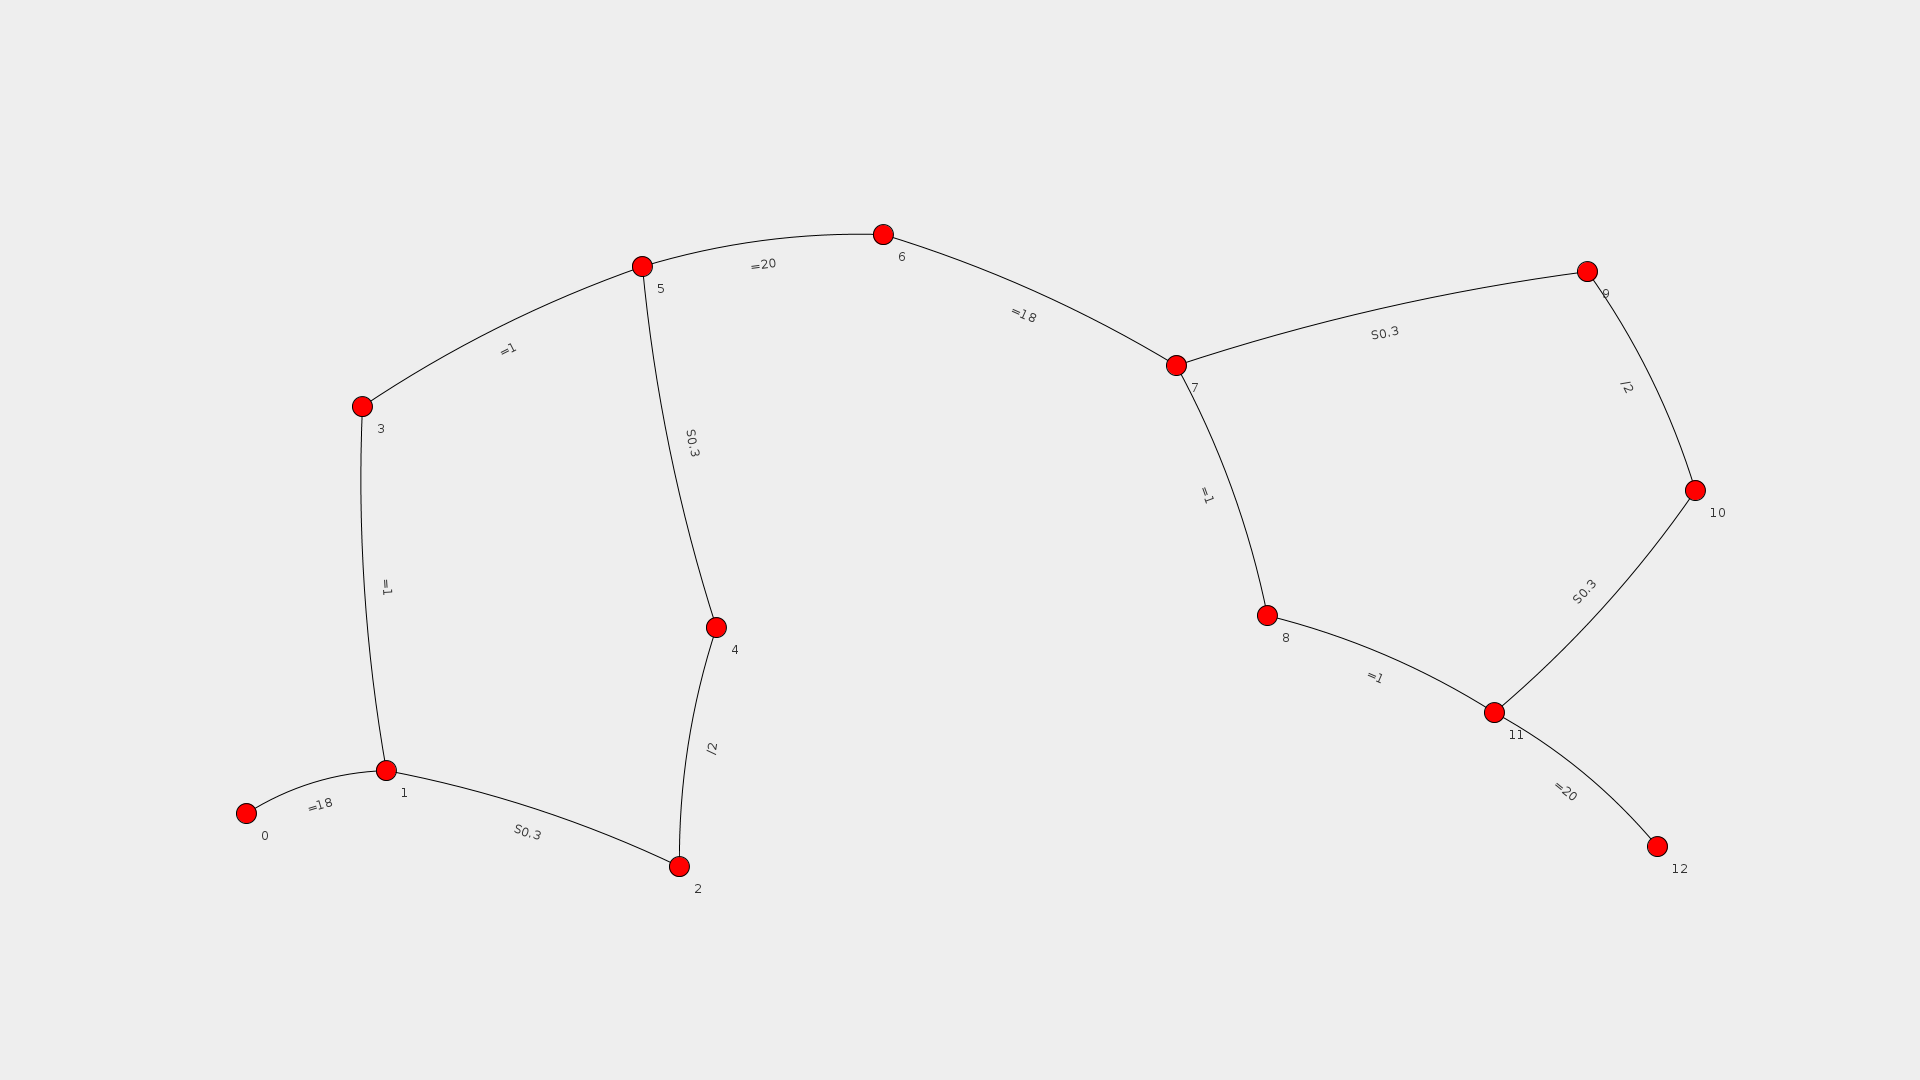
\includegraphics[width=150mm,angle=90]{solution.png}
\caption{RAS DATA SET TOY example territory. Undirected graph, arcs have descriptions.}
\end{figure}

\begin{figure}
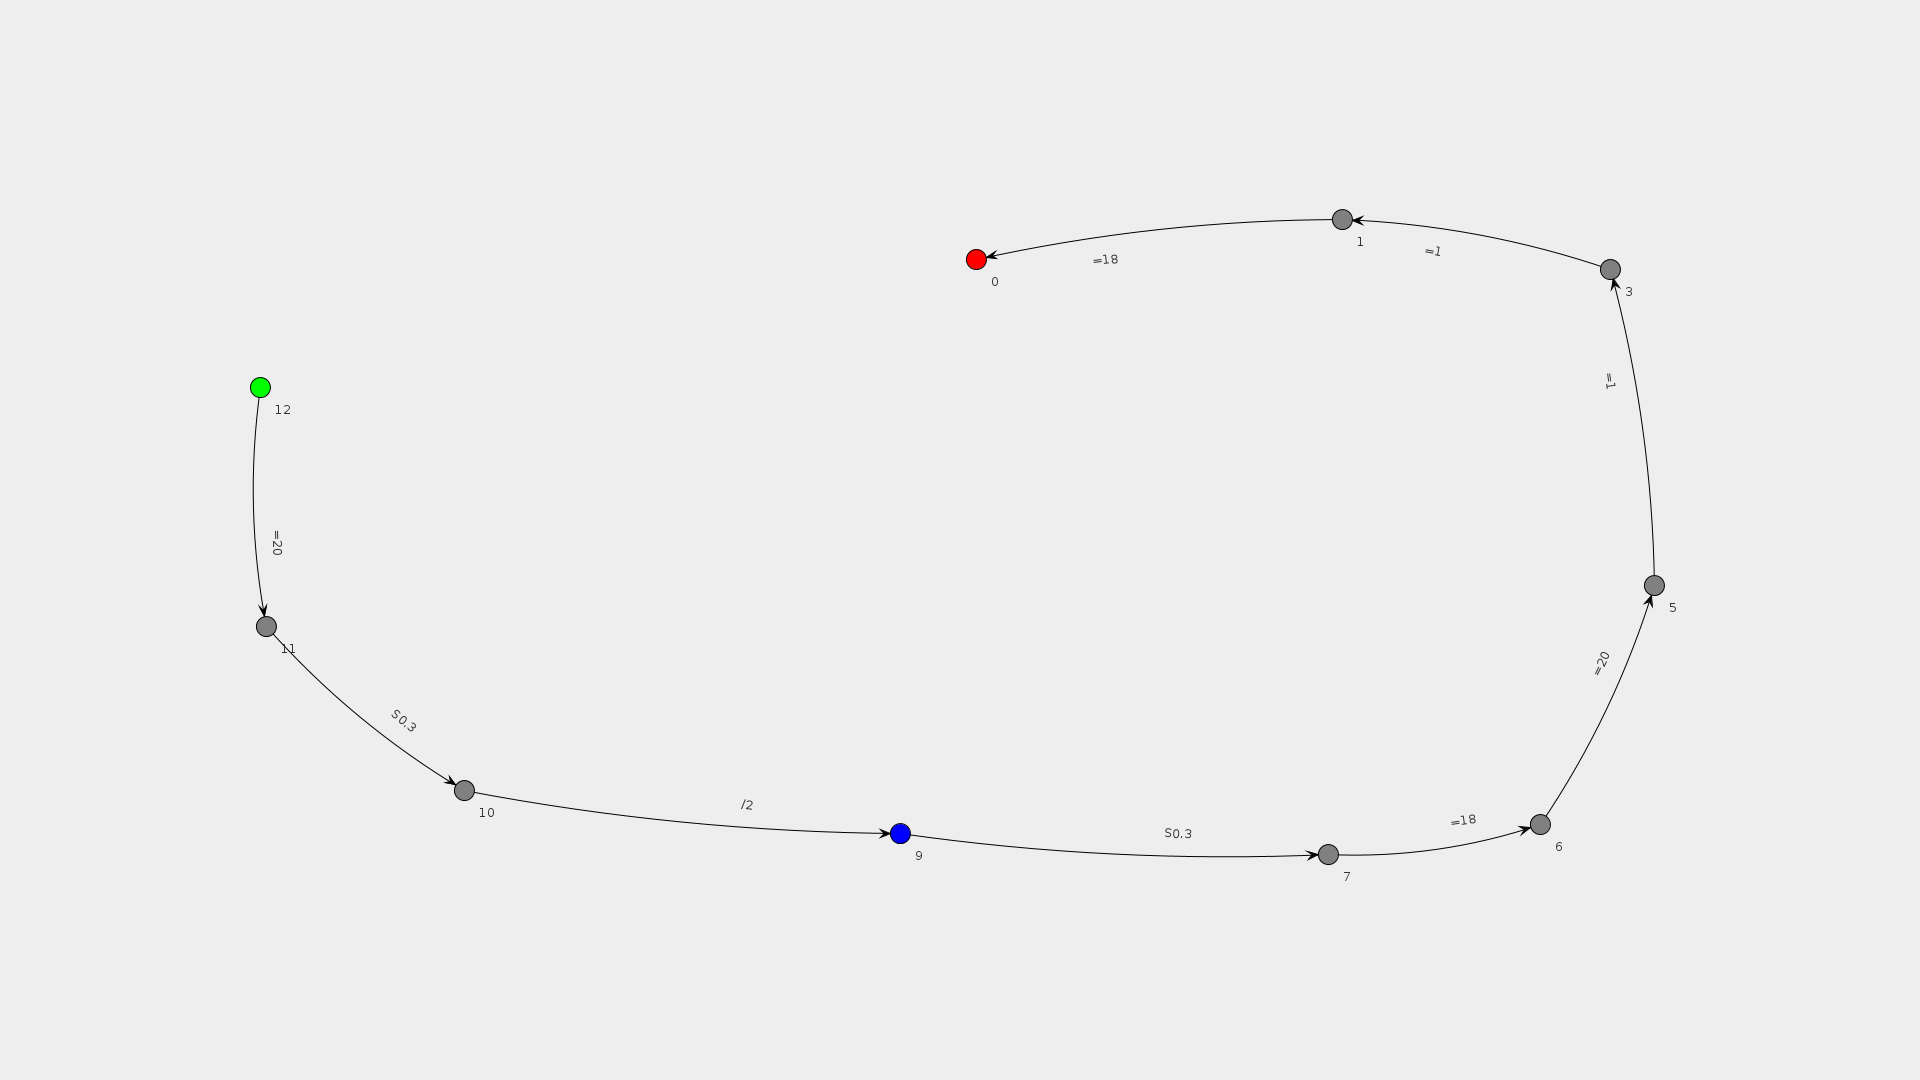
\includegraphics[width=150mm,angle=90]{B1.png}
\centering
\caption{RAS DATA SET TOY example, route of Train B1. Directed graph where green marks the origin, red the destination and blue is where the train is allowed to wait.}
\end{figure}

In this section, we show examples of visualizations that the solution is capable of providing. These visualizations have been rendered on the fly using the JUNG library\footnote{Java Universal Network/Graph framework, http://jung.sourceforge.net}.

\end{document}
